\begin{frame}{Decision tree}
  \begin{description}
    \setlength\itemsep{4mm}
    \item[Rooted tree] where each vertex represents a decision.
    \item[Results] of a decision are represented by the edges to next level.
    \item[Decisions] can connect to other decisions further down the tree.
    \item[Leaves] represent final outcomes.
  \end{description}
\end{frame}



\begin{frame}[fragile]{Sorting three items}
  \begin{center}
    Three items -- $(\alpha, \beta, \gamma )$ \\[1cm]
    \begin{tikzpicture}[->,>=stealth',level/.style={sibling distance = 5cm/#1, level distance = 1.5cm}]
      \tikzset{every node/.style={align=center}}
      \node {\footnotesize $\alpha < \beta$}
        child { node {\footnotesize $\beta < \gamma$}
          child { node {\footnotesize $\alpha < \gamma$}
            child { node {\footnotesize $\alpha \beta \gamma$} edge from parent [->] node [left] {\tiny y} }
            child { node {\footnotesize $n/a$} edge from parent [->] node [right] {\tiny n} }
            edge from parent [->] node [left] {\tiny y} 
          } 
          child { node {\footnotesize $\alpha < \gamma$}
            child { node {\footnotesize $\alpha \gamma \beta$} edge from parent [->] node [left] {\tiny y} }
            child { node {\footnotesize $\gamma \alpha \beta$} edge from parent [->] node [right] {\tiny n} }
            edge from parent [->] node [right] {\tiny n} 
          }
          edge from parent [->] node [left] {\tiny y} 
        }
        child { node {\footnotesize $\beta < \gamma$}
          child { node {\footnotesize $\alpha < \gamma$}
            child { node {\footnotesize $\beta \alpha \gamma$} edge from parent [->] node [left] {\tiny y} }
            child { node {\footnotesize $\beta \gamma \alpha$} edge from parent [->] node [right] {\tiny n} }
            edge from parent [->] node [left] {\tiny y}
          }
          child { node {\footnotesize $\alpha < \gamma$}
            child { node {\footnotesize $n/a$} edge from parent [->] node [left] {\tiny y} }
            child { node {\footnotesize $\gamma \beta \alpha$} edge from parent [->] node [right] {\tiny n} }
            edge from parent [->] node [right] {\tiny n} 
          }
          edge from parent [->] node [right] {\tiny n} 
        };
			\end{tikzpicture}
  \end{center}
\end{frame}


\begin{frame}[fragile]{Decision tree for bubble sort with three items}
  \begin{center}
    Three items -- $(\alpha, \beta, \gamma )$ \\[1cm]
    \begin{tikzpicture}[->,>=stealth',level/.style={sibling distance = 5cm/#1, level distance = 1.5cm}]
      \tikzset{every node/.style={align=center}}
      \node {\footnotesize $x_1 < x_2$ \color{darkgray} ($\alpha \beta \gamma$)}
        child { node {\footnotesize $x_2 < x_3$ \color{darkgray} ($\alpha \beta \gamma$)}
          child { node {\footnotesize $x_1 < x_2$ \color{darkgray} ($\alpha \beta \gamma$)}
            child { node {\footnotesize $\alpha \beta \gamma$} edge from parent [->] node [left] {\tiny y} }
            child { node {\footnotesize $n/a$} edge from parent [->] node [right] {\tiny n} }
            edge from parent [->] node [left] {\tiny y} 
          } 
          child { node {\footnotesize $x_1 < x_2$ \color{darkgray} ($\alpha \gamma \beta$)}
            child { node {\footnotesize $\alpha \gamma \beta$} edge from parent [->] node [left] {\tiny y} }
            child { node {\footnotesize $\gamma \alpha \beta$} edge from parent [->] node [right] {\tiny n} }
            edge from parent [->] node [right] {\tiny n} 
          }
          edge from parent [->] node [left] {\tiny y} 
        }
        child { node {\footnotesize $x_2 < x_3$ \color{darkgray} ($\beta \alpha \gamma$)}
          child{ node {\footnotesize $x_1 < x_2$ \color{darkgray} ($\beta \alpha \gamma$)}
            child { node {\footnotesize $\beta \alpha \gamma$} edge from parent [->] node [left] {\tiny y} }
            child { node {\footnotesize $n/a$} edge from parent [->] node [right] {\tiny n} }
            edge from parent [->] node [left] {\tiny y} 
          }
          child { node {\footnotesize $x_1 < x_2$ \color{darkgray} ($\beta \gamma \alpha$)}
            child { node {\footnotesize $\beta \gamma \alpha$} edge from parent [->] node [left] {\tiny y} }
            child { node {\footnotesize $\gamma \beta \alpha$} edge from parent [->] node [right] {\tiny n} }
            edge from parent [->] node [right] {\tiny n} 
          }
          edge from parent [->] node [right] {\tiny n} 
        };
			\end{tikzpicture}
  \end{center}
\end{frame}


\begin{frame}{Heap sort}
  \vspace{4mm}
  \begin{description}
    \setlength\itemsep{4mm}
    \item[Comparison] sorting algorithm.
    \item[Better] worst case performance than quicksort: \(O(n \log n)\).
    \item[Same] average performance as quicksort: \(O(n \log n)\) versus \(O(n^2)\).
    \item[Uses] trees to sort elements.
    \item[Heap] is a binary tree where label of each parent is less than or equal to its children's.
  \end{description}
\end{frame}

\begin{frame}[fragile]{Heapsort initial tree}
  \begin{center}
    $(x_{01},x_{02},x_{03},x_{04},x_{05},x_{06},x_{07},x_{08},x_{09},x_{10},x_{11},x_{12})$ \\[1cm]
    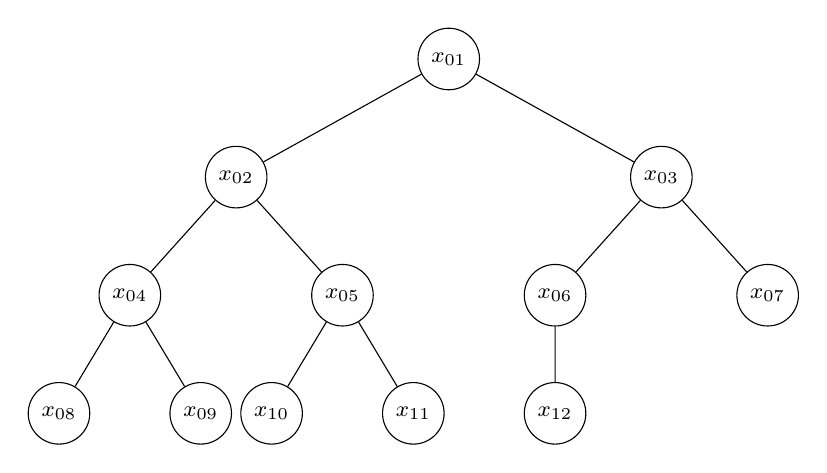
\begin{tikzpicture}[level/.style={sibling distance = 54mm/#1, level distance = 15mm}]
      \tikzset{every node/.style={align=center,draw,circle}}
      \node {\footnotesize $x_{01}$}
        child { node {\footnotesize $x_{02}$}
          child { node {\footnotesize $x_{04}$}
            child { node {\footnotesize $x_{08}$} }
            child { node {\footnotesize $x_{09}$} }
          } 
          child { node {\footnotesize $x_{05}$}
            child { node {\footnotesize $x_{10}$} }
            child { node {\footnotesize $x_{11}$} }
          }
        }
        child { node {\footnotesize $x_{03}$}
          child { node {\footnotesize $x_{06}$}
            child { node {\footnotesize $x_{12}$} }
          } 
          child { node {\footnotesize $x_{07}$} }
        };
			\end{tikzpicture}
  \end{center}
\end{frame}


\begin{frame}[fragile]{Heapsort initial tree}
  \begin{center}
    $(77,23,82,47,65,17,97,85,35,91,61,73)$ \\[1cm]
    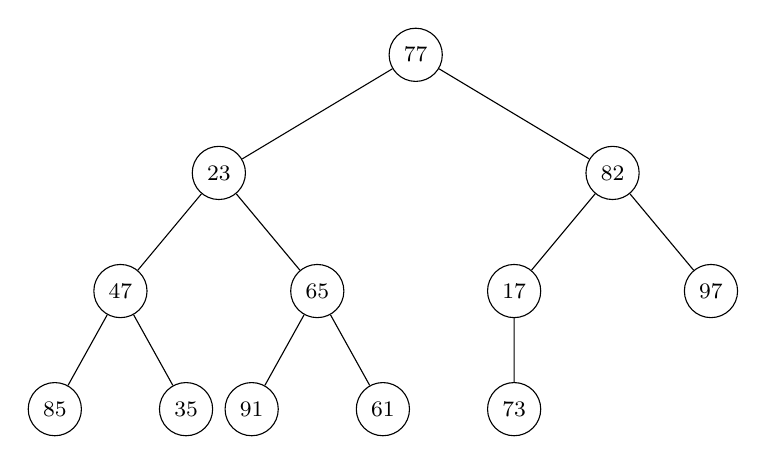
\begin{tikzpicture}[level/.style={sibling distance = 5cm/#1, level distance = 1.5cm}]
      \tikzset{every node/.style={align=center,draw,circle}}
      \node {\footnotesize $77$}
        child { node {\footnotesize $23$}
          child { node {\footnotesize $47$}
            child { node {\footnotesize $85$} }
            child { node {\footnotesize $35$} }
          } 
          child { node {\footnotesize $65$}
            child { node {\footnotesize $91$} }
            child { node {\footnotesize $61$} }
          }
        }
        child { node {\footnotesize $82$}
          child { node {\footnotesize $17$}
            child { node {\footnotesize $73$} }
          } 
          child { node {\footnotesize $97$} }
        };
			\end{tikzpicture}
  \end{center}
\end{frame}


\begin{frame}{Tree to a heap}
  \begin{description}
    \setlength\itemsep{4mm}
    \item[Start] at the last parent and move backwards through the other parents as follows.
    \item[Suppose] current parent is $x_r$ and the trees at $x_{2r}$ and $x_{2r+1}$ are already heaps.
    \item[Compare] $x_r$ to .
    \item[If] $x_{2r}$ or $x_{2r+1}$ is smaller than $x_r$ then swap $x_r$ with the smaller child.
    \item[If necessary] apply this procedure to the new child.
  \end{description}
\end{frame}


\begin{frame}[fragile]{Heapsort - the heap}
  \begin{center}
    $(17,23,73,35,61,77,97,85,47,91,65,82)$ \\[2mm]
    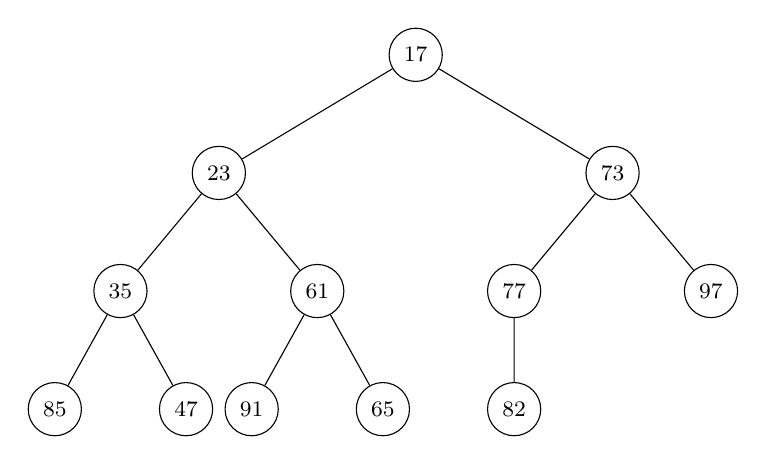
\begin{tikzpicture}[level/.style={sibling distance = 5cm/#1, level distance = 1.5cm}]
      \tikzset{every node/.style={align=center,draw,circle}}
      \node {\footnotesize $17$}
        child { node {\footnotesize $23$}
          child { node {\footnotesize $35$}
            child { node {\footnotesize $85$} }
            child { node {\footnotesize $47$} }
          } 
          child { node {\footnotesize $61$}
            child { node {\footnotesize $91$} }
            child { node {\footnotesize $65$} }
          }
        }
        child { node {\footnotesize $73$}
          child { node {\footnotesize $77$}
            child { node {\footnotesize $82$} }
          } 
          child { node {\footnotesize $97$} }
        };
    \end{tikzpicture} \\[2mm]
    $x_r < x_{2r}$ and $x_r < x_{2r+1}$
  \end{center}
\end{frame}


\begin{frame}{Transforming to a sorted list}
  \begin{description}
    \setlength\itemsep{4mm}
    \item[Start] with and empty list.
    \item[Place] the root of the heap at the end of the list.
    \item[Remove] the last leaf and place it at the root.
    \item[Transform] the tree to a heap again. This is relatively easy since the subtrees at $x_2$ and $x_3$ are already heaps.
    \item[Repeat] until tree is empty.
  \end{description}
  \vspace{4mm}
  $$ (17,23,35,47,61,65,73,77,82,85,91,97) $$
\end{frame}


\begin{frame}{Searching trees and graphs}
  \begin{description}
    \setlength\itemsep{4mm}
    \item[Searching] is often visualised in graph form.
    \item[Usually] on a spanning tree.
    \item[Main methods] for searching through tree are depth-first and breadth-first.
    \item[Pick] one node to start at (the root).
    \item[Depth-first] means you go as far along each branch as possible before going to the next branch.
    \item[Breadth-first] means you visit each vertex at level $i$ before proceeding to level $i+1$.
  \end{description}
\end{frame}


\begin{frame}[fragile]{Depth-first search}
  \begin{center}
    \forestset{declare keylist register={through}, through={}, circles tree/.style={for tree={circle, draw, fill=white, align=center},}, tracing tree/.style={delay={for #1={if phantom={}{through+/.option=name},}},before drawing tree={tikz+/.wrap pgfmath arg={\foreach \i [count=\j, remember=\i as \k] in {##1} \ifnum\j>1 \draw [densely dashed, -Stealth] (\k.west) -- (\i.west)\fi;}{(through)}},}}
    \begin{forest}
      circles tree, tracing tree=tree,%tree breadth-first,
      [$a$
        [$b$
          [$d$
            [$h$]
            [,phantom]
          ]
          [$e$
            [$i$]
            [$j$]
          ]
        ]
        [$c$
          [$f$
            [,phantom]
            [$k$]
          ]
          [$g$]
        ]
      ]
    \end{forest}
  \end{center}
  \citeurl{tex.stackexchange.com/questions/332300}
\end{frame}


\begin{frame}[fragile]{Breadth-first search}
  \begin{center}
    \forestset{declare keylist register={through}, through={}, circles tree/.style={for tree={circle, draw, fill=white, align=center},}, tracing tree/.style={delay={for #1={if phantom={}{through+/.option=name},}},before drawing tree={tikz+/.wrap pgfmath arg={\foreach \i [count=\j, remember=\i as \k] in {##1} \ifnum\j>1 \draw [densely dashed, -Stealth] (\k.west) -- (\i.west)\fi;}{(through)}},}}
    \begin{forest}
      circles tree, tracing tree=tree breadth-first,
      [$a$
        [$b$
          [$d$
            [$h$]
            [,phantom]
          ]
          [$e$
            [$i$]
            [$j$]
          ]
        ]
        [$c$
          [$f$
            [,phantom]
            [$k$]
          ]
          [$g$]
        ]
      ]
    \end{forest}
  \end{center}
  \citeurl{tex.stackexchange.com/questions/332300}
\end{frame}